\section{Theory}
\begin{figure}[htpb!]
    \centering
    \begin{tikzpicture}[scale=1.3]
        \tikzmath{\m = 0;}
        \draw[->]  (-1,0) -- (4,0) node[right] {$x$};
        \draw[->]  (0,-1.1) -- (0,4) node[right] {$y$};
        \draw[very thin, opacity=0.3] (-3.9,-1.1) grid (3.9,3.9);
        
        \foreach \x in {-3,-2,-1,1,2,3}
        \draw (\x, 0.05) -- (\x, -0.05) node[below, font=\tiny] {\x};
        
        \foreach \sgm/\col in {0.2/violet, 0.5/red!80!black, 1/teal, 2/orange!90!black}
            {    
                \draw[domain=-4:4, samples=250, smooth, \col]
                plot (\x, {1/(\sgm*sqrt(2*pi))*exp(-((\x-\m)*(\x-\m))/(2*\sgm*\sgm))});
            }
    \end{tikzpicture}
    \caption{Normal PDF $\frac{1}{\sqrt{2\pi}\sigma}e^{-\frac{(x-\mu)^2}{2\sigma^2}}$}
\end{figure}

\subsection{Central limit theorem}
For $X_1, ..., X_n \overset{iid}{\sim} X$ we have:
\[\frac{\sum_{i=1}^{n} X_i - n\E[X]}{\sqrt{n\var(X)}} \overset{d}{\rightarrow} \mathcal{N}(0, 1)\]
meaning the CDF of the normalized empirical mean converges to the CDF of the standard normal distribution. Using this theorem we run the approximation using the binomial distribution with $p = 0.3$ and $n = 1000$. Figure \ref{fig:cdf qq} illustrates the approximation result.

\begin{figure}[htpb!]
    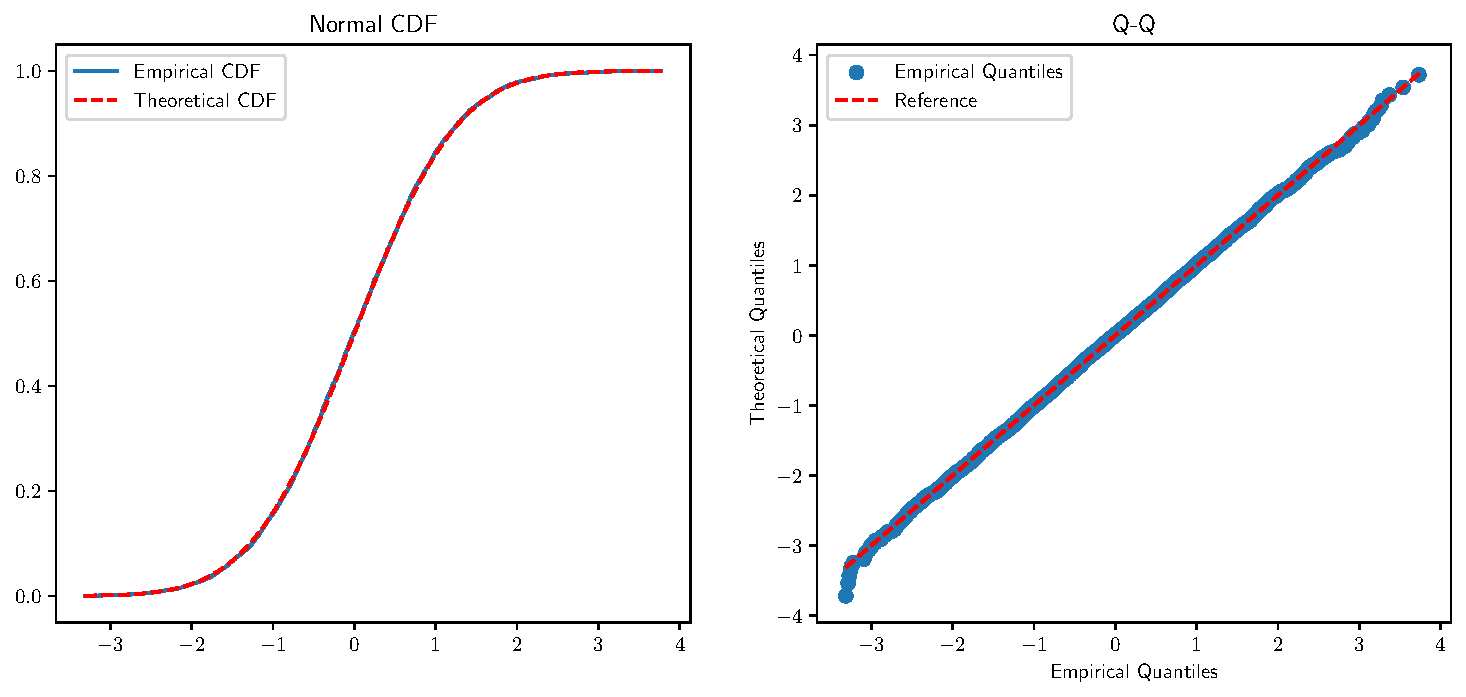
\includegraphics[width = \textwidth]{cdf_qq.pdf}
    \caption{CDF and Q-Q plot}
    \label{fig:cdf qq}
\end{figure}

\subsection{Approximation quality}
We want to estimate how accurate is the estimate:
\[F_n(t)
    = \frac{1}{n} \sum_{i=1}^{n} \I_{X_i \leq t}
    = \frac{1}{n} \sum_{i=1}^{n} \I_{(-\infty,t]}(X_i)\]

The estimate is unbiased since:
\begin{equation} \label{eq:unbiasedness}
    \begin{split}    
        \E \left[\frac{1}{n} \sum_{i=1}^{n} \I_{X_i \leq t}\right]
        = \frac{1}{n} \sum_{i=1}^{n} \E \left[\I_{X_i \leq t}\right]
         & \overset{*}{=} \frac{1}{n} \sum_{i=1}^{n} \P (X_i \leq t)
        \\ &\overset{**}{=} \frac{1}{n} \sum_{i=1}^{n} \P (X \leq t)
        = \P (X \leq t)
    \end{split}
\end{equation}
where $*$ holds since as we integrate the indicator function we get the probability of the event, and $**$ holds since $X_i \sim X$.

Each $\I_{X_i \leq t}$ is bounded by $[0, 1]$, so we can use Hoeffding's inequality to get a bound on the probability of the estimate being far from the true value:
\begin{equation} \label{eq:hoeffding bound}
    \P \left(\left|\frac{1}{n} \sum_{i=1}^{n} \I_{X_i \leq t} - \P (X \leq t)\right| \geq \delta\right)
    = \P \left(\left|\frac{1}{n} \sum_{i=1}^{n} \I_{X_i \leq t} - F(t)\right| \geq \delta\right)
    \leq 2 e^{-2 n \delta^2}
\end{equation}

Figure~\ref{fig:hoeffding} illustrates the bound for different values of $\delta$.
\begin{figure}[htpb!]
    \centering
    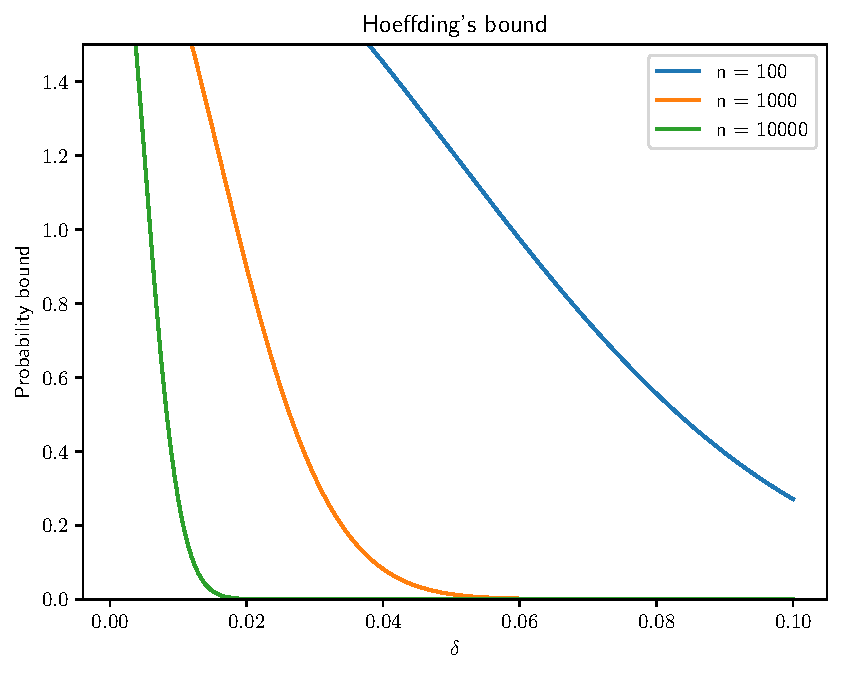
\includegraphics[width = 0.7\textwidth]{hoeffding.pdf}
    \caption{Hoeffding's inequality bound}
    \label{fig:hoeffding}
\end{figure}

For the almost sure convergence refer to \href{https://en.wikipedia.org/wiki/Glivenko%E2%80%93Cantelli_theorem}{Glivenko---Cantelli theorem}, which states the following:
\begin{theorem}[Glivenko---Cantelli theorem] \label{thm:glivenko-cantelli}
    Let $X_1, X_2, ... \overset{iid}{\sim} X$ and $F(x)$ be CDF of $X$. Moreover let $F$ be continuous. Then we have:
    \[\P \left(\sup_{t \in \R} \left|F_n(t) - F(t) \right| \to 0 \right) = 1\]
    where
    \[F_n(t) = \frac{1}{n} \sum_{i=1}^{n} \I_{(-\infty,t]}(X_i)\]
\end{theorem}

\begin{proof}[Proof of Theorem~\ref{thm:glivenko-cantelli}]
    Fix $-\infty = x_0 \leq x_1 \leq ... \leq x_m = \infty$, s.t. $F(x_k) + 1/m = F(x_{k + 1})$ (using intermediate value theorem assuming $F$ is continuous) for all $k \in \{0, ..., m - 1\}$. Then if $x \in [x_{k-1}, x_k]$ by monotonicity of $F_n$ and $F$ we have:
    \begin{itemize}    
        \item $F_n(x) - F(x)
                  \geq F_n(x_{k-1}) - F(x_{k})
                  = F_n(x_{k-1}) - F(x_{k-1}) - 1/m$
        \item $F_n(x) - F(x)
                  \leq F_n(x_{k}) - F(x_{k - 1})
                  = F_n(x_{k}) - F(x_{k}) + 1/m$
    \end{itemize}
    
    Thus we have that for each $x \in \R$ there exists $k \in \{1, ..., m\}$ s.t. $x \in [x_{k-1}, x_k]$ hence:
    \begin{equation} \label{eq:epsilon boundedness}
        \begin{split}    
            \sup_{x \in \R} |F_n(x) - F(x)| \leq \max_{k \in \{0, ..., m\}} |F_n(x_{k}) - F(x_{k})| + 1/m
        \end{split}
    \end{equation}
    
    If we now suppose that for some $\omega \in \Omega$:
    \[\sup_{x \in \R} |F_n(x)(\omega) - F(x)| > \varepsilon + 1/m\]
    then by \eqref{eq:epsilon boundedness} we have that:
    \[\max_{k \in \{0, ..., m\}} |F_n(x_{k})(\omega) - F(x_{k})| > \varepsilon\]
    thus:
    \begin{equation} \label{eq:probability monotonicity}
        \P\left(\sup_{x \in \R} |F_n(x) - F(x)| > \varepsilon + 1/m \text{ i.o.} \right)
        \leq \P\left(\max_{k \in \{0, ..., m\}} |F_n(x_{k}) - F(x_{k})| > \varepsilon \text{ i.o.} \right)
    \end{equation}
    as $\forall n \in \N$ for which the left hand side event occurs the right hand side event event occurs as well.
    
    Since $F_n(t)$ is the sum of $n$ independent random variables, we can use the strong law of large numbers (the estimate is unbiased \eqref{eq:unbiasedness}, $\I_{(-\infty,t]}(X_i)$ are independent) to get that for each $k \in \{0, ..., m\}$:
    \[\P \left(\lim_{n \to \infty} F_n(x_k) = F(x_k)\right) = 1\]
    
    Thus for each $\varepsilon > 0$ we have:
    \[\P \left(|F_n(x_k) - F(x_k)| > \varepsilon \text{ i.o.}\right) = 0\]
    and by union bound we get:
    \[\P \left(\bigcup_{k=0}^{m} \{|F_n(x_k) - F(x_k)| > \varepsilon \text{ i.o.}\}\right)
        \leq \sum_{k=0}^{m} \P \left(|F_n(x_k) - F(x_k)| > \varepsilon \text{ i.o.}\right) = 0\]
    
    \begin{claim} \label{cl:limsup commutativity}
        Let ${(A_n)}_{n \in \N}, {(B_n)}_{n \in \N} \in \mathcal{F}$ be two sequences of events. Then we have:
        \[\limsup_{n \to \infty} (A_n \cup B_n)
            = \limsup_{n \to \infty} A_n \cup \limsup_{n \to \infty} B_n\]
    \end{claim}
    \begin{proof}[Proof of Claim~\ref{cl:limsup commutativity}]
        \[\limsup_{n \to \infty} (A_n \cup B_n)
            = \bigcap_{n=1}^{\infty} \bigcup_{m=n}^{\infty} (A_m \cup B_m)
            \overset{*}{=} \bigcap_{n=1}^{\infty} \left(\left(\bigcup_{m=n}^{\infty} A_m\right) \cup \left(\bigcup_{m=n}^{\infty} B_m\right) \right)\]
        where $*$ holds by associativity and commutativity of union.
        
        Denote:
        \[\tilde{A}_n = \bigcup_{m=n}^{\infty} A_m \quad \tilde{B}_n = \bigcup_{m=n}^{\infty} B_m\]
        
        We have that $\tilde{A}_n$ and $\tilde{B}_n$ are decreasing sequences of events.
        
        \begin{enumerate}[align=left]
            \item[``$\subset$''] Suppose:
                  \[\omega \in \bigcap_{n=1}^{\infty} (\tilde{A}_n \cup \tilde{B}_n)
                      \Rightarrow \omega \in \tilde{A}_n \cup \tilde{B}_n \; \forall n \in \N\]
                  meaning for each $n \in \N$ $\omega \in \tilde{A}_n$ or $\omega \in \tilde{B}_n$. Assume that for some $k \in \N$ $\omega \notin \tilde{A}_k$. Then for any $n > k$ we have that $\omega \notin \tilde{A}_n$, so we must have $\omega \in \tilde{B}_n$ for all $n > k$. Since $\tilde{B}_n$ is decreasing:
                  \[\omega \in \bigcap_{n = k}^{\infty} \tilde{B}_n = \bigcap_{n = 1}^{\infty} \tilde{B}_n\]
                  
                  Otherwise if $\omega \in \tilde{A}_n$ for all $n \in \N$ we have:
                  \[\omega \in \bigcap_{n = 1}^{\infty} \tilde{A}_n\]
                  which implies:
                  \[\omega \in \left(\bigcap_{n = 1}^{\infty} \tilde{A}_n \right) \cup \left(\bigcap_{n = 1}^{\infty} \tilde{B}_n \right)\]
            \item[``$\supset$''] Suppose:
                  \[\omega \in \left(\bigcap_{n = 1}^{\infty} \tilde{A}_n \right) \cup \left(\bigcap_{n = 1}^{\infty} \tilde{B}_n \right)\]
                  which means either $\omega \in \bigcap_{n = 1}^{\infty} \tilde{A}_n$ or $\omega \in \bigcap_{n = 1}^{\infty} \tilde{B}_n$. In the first case we have that $\omega \in \tilde{A}_n$ for all $n \in \N$, which implies $\omega \in \tilde{A}_n \cup \tilde{B}_n$ for all $n \in \N$. The second case is analogous.
        \end{enumerate}
    \end{proof}
    
    With the Claim~\ref{cl:limsup commutativity} we can rewrite the union of events as:
    \begin{align}    
        \left\{\max_{k \in \{0, ..., m\}} |F_n(x_k) - F(x_k)| > \varepsilon \text{ i.o.} \right\}
         & = \left\{\left(\bigcup_{k \in \{0, ..., m\}} |F_n(x_k) - F(x_k)| > \varepsilon \right) \text{ i.o.}\right\} \notag
        \\ &= \left\{\bigcup_{k \in \{0, ..., m\}} \left(|F_n(x_k) - F(x_k)| > \varepsilon \text{ i.o.} \right)\right\} \label{eq:infinitely often bounded}
    \end{align}
    
    Equation~\ref{eq:probability monotonicity} together with equation~\ref{eq:infinitely often bounded} gives us:
    \[\P \left(\sup_{x \in \R}|F_n(x) - F(x)| > \varepsilon + 1/m \text{ i.o.}\right) = 0\]
    
    Finally since $m$ is arbitrary we can choose $m \geq 2 / \tilde{\varepsilon}$ and $\varepsilon = \tilde{\varepsilon} / 2$ to get:
    \[\P \left(\sup_{x \in \R}|F_n(x) - F(x)| > \tilde{\varepsilon} \text{ i.o.}\right) = 0 \quad \forall \tilde{\varepsilon} > 0\]
    which is equivalent to:
    \[\P \left(\sup_{x \in \R}|F_n(x) - F(x)| \to 0\right) = 1\]
\end{proof}

\begin{remark}    
    The proof translates bounding an uncountable set of points to bounding a finite set of points. This result is of interest since it shows uniform convergence of the empirical CDF including the tails of the distribution, which is important for statistical inference.
\end{remark}

\begin{theorem}[Rate of convergence] \label{thm:rate of convergence}
    Let $X_1, X_2, ... \overset{iid}{\sim} X$ and $F(x)$ be CDF of $X$. Moreover let $F$ be continuous. Then we have:
    \[\P \left(\sup_{t \in \R} \left|F_n(t) - F(t) \right| \geq \delta\right)
        \leq 4\left(1 + \frac{1}{\delta}\right)e^{-\frac{n\delta^2}{2}}, \quad \forall \delta > 0\]
    where
    \[F_n(t) = \frac{1}{n} \sum_{i=1}^{n} \I_{(-\infty,t]}(X_i)\]
\end{theorem}
\begin{proof}[Proof of Theorem~\ref{thm:rate of convergence}]
    Choose the points $x_0, ..., x_m$ as in the proof of Theorem~\ref{thm:glivenko-cantelli}. Then using the bound \eqref{eq:hoeffding bound} we have:
    \[\P \left(\left|\frac{1}{n} \sum_{i=1}^{n} \I_{X_i \leq t} - F(t)\right| \geq \varepsilon\right)
        = \P \left(\left|F_n(t) - F(t)\right| \geq \varepsilon\right)
        \leq 2e^{-2 n \varepsilon^2}\]
    for all $t \in \R$ including the points $x_0, ..., x_m$. Then using the union bound we have:
    \[\P \left(\max_{k \in \{0, ..., m\}} \left|F_n(x_k) - F(x_k)\right| \geq \varepsilon\right)
        \leq 2(m+1)e^{-2 n \varepsilon^2}\]
    
    Similarly to equation~\ref{eq:probability monotonicity} we have that:
    \begin{align*}    
        \P & \left(\sup_{x \in \R} \left|F_n(x) - F(x)\right| \geq \varepsilon + 1/m\right)
        \\ &\leq \P \left(\max_{k \in \{0, ..., m\}} \left|F_n(x_k) - F(x_k)\right| \geq \varepsilon\right)
        \leq 2(m+1)e^{-2 n \varepsilon^2}
    \end{align*}
    which holds for any $m \in \N$.
    
    Now fix $\delta > 0$, choose $m = \lceil 2/\delta \rceil$, and substitute $\varepsilon = \delta/2$ into the inequality above:
    \[\P \left(\sup_{x \in \R} \left|F_n(x) - F(x)\right| \geq \frac{\delta}{2} + \frac{1}{m}\right)
        \leq 2(m + 1)e^{-\frac{n\delta^2}{2}}\]
    
    Since $m = \lceil 2/\delta \rceil$, we have $1/m \leq \delta/2$, hence:
    \[\left\{\sup_{x \in \R} \left|F_n(x) - F(x)\right| \geq \delta\right\}
        \subseteq \left\{\sup_{x \in \R} \left|F_n(x) - F(x)\right| \geq \frac{\delta}{2} + \frac{1}{m}\right\}\]
    and therefore:
    \[\P \left(\sup_{x \in \R} \left|F_n(x) - F(x)\right| \geq \delta\right)
        \leq 2(m + 1)e^{-\frac{n\delta^2}{2}}\]
    
    Finally, using $m = \lceil 2/\delta \rceil \leq 2/\delta + 1$, we get:
    \[2(m + 1) \leq 2\left(\frac{2}{\delta} + 2\right) = 4\left(1 + \frac{1}{\delta}\right)\]
    so:
    \[\P \left(\sup_{x \in \R} \left|F_n(x) - F(x)\right| \geq \delta\right)
        \leq 4\left(1 + \frac{1}{\delta}\right)e^{-\frac{n\delta^2}{2}}\]
\end{proof}

\begin{figure}[htpb!]
    \centering
    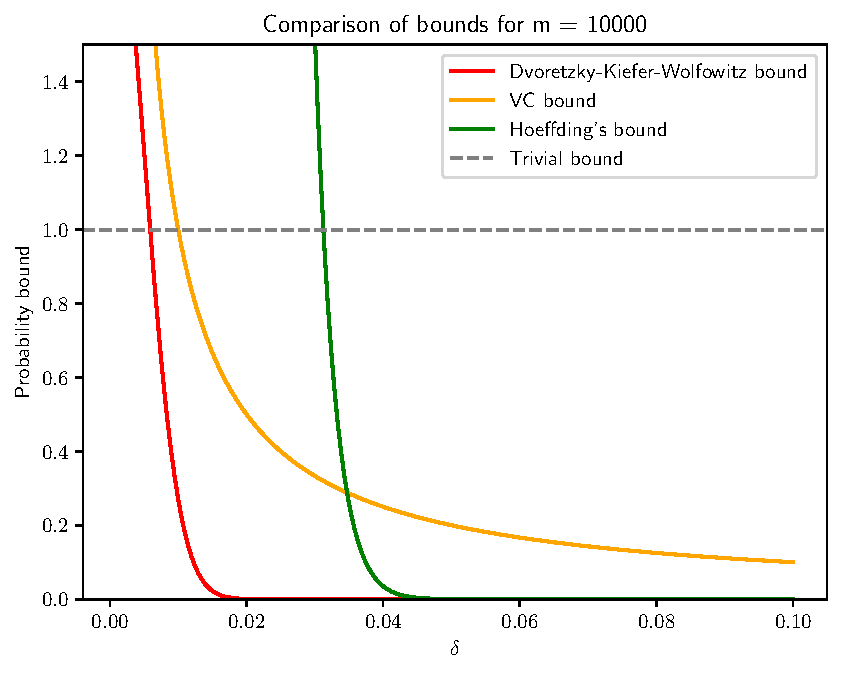
\includegraphics[width = 0.7\textwidth]{bounds_comparison.pdf}
    \caption{\centering Bounds comparison: Hoeffding's inequality (Theorem~\ref{thm:rate of convergence}), Dvoretzky---Kiefer---Wolfowitz inequality (Remark~\ref{rem:dkw}), VC theory bound (Remark~\ref{rem:vc bound})}
    \label{fig:bounds comparison}    
\end{figure}

\begin{remark} \label{rem:dkw}
    For the tighter bound refer to \href{https://en.wikipedia.org/wiki/Dvoretzky%E2%80%93Kiefer%E2%80%93Wolfowitz_inequality}{Dvoretzky---Kiefer---Wolfowitz inequality}, which states the following:
    \[\P \left(\sup_{t \in \R} \left|F_n(t) - F(t) \right| \geq \delta\right)
        \leq 2e^{-2n\delta^2}, \quad \forall \delta \geq 0\]
    
    Note that this is the same exact bound as in \eqref{eq:hoeffding bound} but uniform over all $t \in \R$
\end{remark}

\newcommand{\loss}{\operatorname{\mathscr{L}}}
\begin{remark} \label{rem:vc bound}
    By VC theory we have that the hypothesis class:
    \[\mathcal{H} = \{h_t = \I_{(-\infty, t]}: t \in \R\}\]
    has VC dimension $d = 1$. Note that for the distribution $\mathcal{D}$ induced by $(X, 0)$, where $X$ is a random variable and $0$ is the label, we have that the training loss for the sample $\mathcal{T} = ((X_1, 0), ..., (X_n, 0)) \overset{iid}{\sim} \mathcal{D}$ is given by:
    \[\loss_{\mathcal{T}} = \frac{1}{n} \sum_{i=1}^{n} \ell_{0-1}(\I_{(-\infty, t]}(X_i), 0)
        = \frac{1}{n} \sum_{i=1}^{n} \I_{(-\infty, t]}(X_i)
        = F_n(t)\]
    
    The true loss is given by:
    \[\loss_{\mathcal{D}}(h_t) 
        = \E_{(X, 0) \sim \mathcal{D}}[\ell_{0-1}(\I_{(-\infty, t]}(X), 0)]
        = \E_{X \sim \mathcal{D}}[\I_{(-\infty, t]}(X)]
        = \P(X \leq t)
        = F(t)\]
    
    By Fundamental Theorem of Statistical Learning Theory for any distribution $\mathcal{D}$:
    \[\E \left[\sup_{h \in \mathcal{H}} \left|\loss_{\mathcal{T}}(h) - \loss_{\mathcal{D}}(h) \right| \right]
        = \E \left[\sup_{t \in \R} |F_n(t) - F(t)| \right]
        \leq C\sqrt{\frac{\mathrm{VC}(\mathcal{H})}{n}}\]
    for some constant $C > 0$.
    
    By Markov's inequality we have that for any $\delta > 0$:
    \[\P \left(\sup_{t \in \R} |F_n(t) - F(t)| \geq \delta\right)
        \leq \frac{\E\left[\sup_{t \in \R} |F_n(t) - F(t)| \right]}{\delta}
        \leq \frac{C\sqrt{\frac{\mathrm{VC}(\mathcal{H})}{n}}}{\delta}
        = C\sqrt{\frac{1}{n\delta^2}}\]
\end{remark}